% !TeX program = xelatex
% Chinese counterpart of pricai2026_submission_16p.tex. The English 16-page version is kept unchanged.
\documentclass[10pt,a4paper,UTF8,fontset=fandol]{ctexart}

\usepackage{amsmath,amssymb}
\usepackage{booktabs,multirow,array}
\usepackage{threeparttable}
\usepackage{graphicx}
\usepackage{geometry}
\usepackage{hyperref}

\geometry{left=1.85cm,right=1.85cm,top=2.0cm,bottom=2.0cm}
\graphicspath{{../}}
\hypersetup{colorlinks=true,linkcolor=black,citecolor=black,urlcolor=blue,hypertexnames=false}
\emergencystretch=2em

\setlength{\parskip}{0pt}
\setlength{\parindent}{2em}
\setlength{\textfloatsep}{6pt plus 1pt minus 2pt}
\setlength{\floatsep}{5pt plus 1pt minus 2pt}
\setlength{\intextsep}{5pt plus 1pt minus 2pt}
\setlength{\abovedisplayskip}{4pt plus 1pt minus 1pt}
\setlength{\belowdisplayskip}{4pt plus 1pt minus 1pt}
\setlength{\abovedisplayshortskip}{3pt plus 1pt minus 1pt}
\setlength{\belowdisplayshortskip}{3pt plus 1pt minus 1pt}
\renewcommand{\arraystretch}{1.04}

\makeatletter
\renewcommand{\bfdefault}{m}
\makeatother

\ctexset{
  section={format=\Large\rmfamily},
  subsection={format=\large\rmfamily},
  subsubsection={format=\normalsize\rmfamily}
}

\newenvironment{tightitemize}{%
  \begin{itemize}\setlength{\itemsep}{1pt}\setlength{\parskip}{0pt}\setlength{\parsep}{0pt}}{\end{itemize}}
\newenvironment{tightenumerate}{%
  \begin{enumerate}\setlength{\itemsep}{1pt}\setlength{\parskip}{0pt}\setlength{\parsep}{0pt}}{\end{enumerate}}

\begin{document}

\begin{center}
{\Large 边缘计算中信任流驱动的可信联邦关键技术研究\par}
\vspace{4pt}
{\large Trust Flow-Driven Trusted Federated Learning in Edge Computing: A Study on Key Technologies\par}
\vspace{8pt}
{匿名作者\par}
\end{center}

\begin{abstract}
联邦学习（FL）通过避免原始数据迁移来支持边缘智能协同训练，但开放式边缘参与也使聚合过程暴露于不可信执行、模型投毒、隐蔽后门以及严重 Non-IID 偏移等风险之下。现有鲁棒聚合方法往往依赖更严格的阈值来拒绝恶意更新，却容易同时剔除合法的长尾客户端。本文提出一种信任流驱动的可信联邦学习框架，将硬件锚定准入、运行时信任证据、双流信誉演化和风险门控分层聚合联系起来。该方法通过历史性能流和瞬时风险流分离长期效用与短期攻击风险，再利用按层门控、裁剪和幸存者权重重归一化，在抑制投毒更新的同时保留有价值的异构贡献。基于 Flower/PyTorch 的 CIFAR-10 实验包含 20 个准入客户端、6 类混合攻击和 5 次重复运行；结果表明，在 30\% 恶意设置下，该方法达到 92.31\% 的准确率和 10.21\% 的 ASR，永久封禁误杀率接近零。
\end{abstract}

\noindent\textbf{关键词：} 联邦学习；边缘计算；可信执行环境；风险建模；分层聚合；后门防御

\section{引言}

联邦学习通过参数交换训练全局模型，并将数据保留在边缘设备本地\cite{kairouz2021flsurvey,mcmahan2017fedavg}。这一范式适合边缘智能场景，但当客户端身份、执行完整性和更新语义无法完全可信时，聚合阶段会变得脆弱。实际边缘网络还同时存在设备异构和强偏斜数据分布，因此鲁棒聚合必须区分恶意偏移和合法长尾更新。在复合攻击下，这一区分更加困难，因为攻击者可能提交投毒参数、注入定向后门，或利用跨轮伪装降低可见异常。

已有工作从不同角度处理这一问题。Krum 和 Trimmed Mean 等几何或统计防御会剔除离群更新\cite{blanchard2017krum,yin2018byzantine}；FLTrust、FoolsGold、RaSA 以及相关检测方案则利用干净参考、相似性历史或自适应信任机制\cite{cao2021fltrust,fung2020foolsgold,wang2025rasa,dou2025toward,wang2024federated}。面向后门的防御进一步考察触发器行为或合谋模式\cite{bagdasaryan2020backdoor,wang2019neuralcleanse,flpurifier,roseagg,shieldfl}。这些机制仍面临两类反复出现的张力：静态软件检查不能保证本地执行确实真实；过强过滤又容易将 Non-IID 长尾更新误判为攻击。TEE 辅助的联邦学习和可信推理系统提供了硬件信任根\cite{liao2024verifiable,zhang2025rppfl,r1_tee_integrity,r5_tee_mitigating,r12_iot_tee,xu2021distributed,yan2024efficient,lu2025tmt}，但客户端准入之后，TEE 本身并不能判断真实训练产生的模型更新是否在语义上安全。

本文提出 \emph{Trust Flow}，一个面向边缘联邦学习的全流程可信聚合框架。其核心思想是让信任证据在准入、审查、时序状态演化和聚合之间持续流动，而不是把每一轮视作孤立的过滤决策。本文贡献如下：
\begin{tightenumerate}
    \item 提出一种 TEE 锚定的动态准入机制，将远程证明式准入证据与运行时行为熵、卡尔曼滤波结合起来。
    \item 提出双流信誉模型，将历史效用与瞬时攻击风险解耦，以缓解恶意召回与永久误杀之间的冲突。
    \item 提出按层风险门控聚合规则，结合差异化准入阈值、动态 L2 裁剪和幸存者权重重归一化。
    \item 在 Non-IID CIFAR-10 与混合攻击设置下完成端到端评估，并补充压力测试与消融实验。
\end{tightenumerate}

\section{背景与相关工作}

\textbf{边缘计算中的联邦学习。} 标准 FL 工作流中，客户端完成本地训练并向服务器提交参数更新，服务器聚合后再分发全局模型。该流程保留了数据本地性，却使服务器高度依赖上传更新的真实性和质量。边缘计算进一步增加了复杂度，因为客户端的算力、通信稳定性和数据分布均存在差异。簇式 FL、自适应剪枝扩展和拆分式联邦学习已被用于处理异构性和资源约束\cite{r9_clustered,fedpe,parallelsfl}。然而，系统越开放、层级越复杂，客户端准入、本地执行和更新聚合周围的攻击面也越大。

\textbf{投毒与后门攻击。} FL 中的攻击主要包括无目标投毒和目标后门。符号翻转、梯度缩放等无目标投毒旨在破坏收敛；标签翻转、触发器后门、干净标签投毒和语义后门则试图保持主任务行为，同时植入定向误分类。后门攻击尤其棘手，因为恶意更新可在方向上接近正常更新，却改变隐藏特征\cite{bagdasaryan2020backdoor,wang2019neuralcleanse}。在多轮训练中，攻击者还可能先正常行为以积累信任，再注入低幅度或间歇式恶意更新。

\textbf{主动防御及其局限。} 鲁棒聚合通常依赖几何距离、坐标级统计、干净锚点或时序相似性。Krum 与 Trimmed Mean 拒绝或抑制离群更新\cite{blanchard2017krum,yin2018byzantine}；FLTrust 使用服务器端干净参考方向\cite{cao2021fltrust}；FoolsGold 利用历史相似性降低 Sybil 影响\cite{fung2020foolsgold}；RaSA 和近期检测框架进一步在边缘辅助场景下调整聚合或安全聚合\cite{wang2025rasa,dou2025toward,wang2024federated}。FLPurifier、RoseAgg 和 ShieldFL 等后门防御提高了对触发器和合谋模式的保护能力\cite{flpurifier,roseagg,shieldfl}。但这些防御对强 Non-IID 分布仍较敏感：阈值严格会增加良性误杀，阈值宽松则会放过隐蔽攻击。

\textbf{TEE 辅助可信训练。} Intel SGX 和 ARM TrustZone 等可信执行环境可提供隔离执行与受保护密钥材料。已有研究展示了 TEE 在可验证推理、鲁棒隐私保护 FL、训练完整性、攻击缓解和工业 IoT 信任共享中的价值\cite{liao2024verifiable,zhang2025rppfl,r1_tee_integrity,r5_tee_mitigating,r12_iot_tee,xu2021distributed,yan2024efficient,lu2025tmt}。不过，TEE 准入不能单独判断一个真实训练过程生成的模型更新是否语义安全。因此，Trust Flow 将硬件根准入与跨轮风险建模、分层鲁棒聚合结合起来。

\section{系统模型与威胁假设}

系统包含中心服务器 $\mathcal{S}$ 与 $K$ 个边缘客户端 $\mathcal{C}=\{c_1,\ldots,c_K\}$。第 $t$ 轮中，通过准入的客户端接收 $W^{(t-1)}$，完成本地训练后上传 $\Delta W_k^{(t)}$，服务器更新 $W^{(t)}=W^{(t-1)}+\mathrm{Agg}(\{\Delta W_k^{(t)}\})$。全局目标为
\begin{equation}
    \min_W \mathcal{L}(W)=\sum_{k=1}^{K}p_k\mathcal{L}_k(W),\quad
    p_k=|\mathcal{D}_k|/\sum_j|\mathcal{D}_j|.
\end{equation}
边缘场景遵循端-边-云工作流：客户端侧负责本地训练和信任证据生成，服务器侧负责更新审查、信任状态演化和安全聚合。

\begin{figure}[t]
    \centering
    
\includegraphics[width=0.84\textwidth]{fig1_system_arch.pdf}
    \caption{TEE 锚定的端-边-云协同架构。}
    \label{fig:system_arch}
\end{figure}

\begin{figure}[t]
    \centering
    
\includegraphics[width=0.80\textwidth]{fig2_threat_model.pdf}
    \caption{复合投毒与渗透威胁模型。}
    \label{fig:threat_model}
\end{figure}

\textbf{威胁模型。} 服务器是诚实但好奇的，并按聚合协议执行。攻击者可控制已准入客户端，并实施标签翻转、触发器后门、干净标签投毒、语义后门、符号翻转和梯度缩放。本文假设恶意客户端比例上界为 $<50\%$。主实验采用 30\% 作为典型高风险设置，并额外报告 50\% 边界压力测试。TEE 被假定能够在宿主操作系统被攻陷时保护证明关键代码和密钥，但不考虑物理探测和高级微架构侧信道攻击。

\textbf{设计目标。} Trust Flow 旨在：（i）在混合投毒和后门攻击下保持收敛；（ii）使合法长尾客户端的永久封禁误杀率（FPR）保持较低；（iii）避免重型密码学开销，同时保持边缘可部署性。图~\ref{fig:system_arch} 和图~\ref{fig:threat_model} 分别概括物理工作流与威胁面。

这些目标相互耦合。纯过滤策略中，增强拒绝规则可以提高恶意召回，却会同时剔除本地分布偏离多数方向的良性客户端；放宽规则能保护长尾客户端，却会让低幅度投毒持续存在。Trust Flow 将该问题视为状态分离问题，而不是简单阈值调参：准入证据、内容质量、历史贡献和瞬时风险在最终分层聚合决策之前始终保持为不同信号。

\section{Trust-Flow 框架}

Trust Flow 将每一轮 FL 划分为四个相互连接的阶段：准入与运行时信任评估、基于参考的内容审查、双流状态演化以及风险门控分层聚合。图~\ref{fig:framework} 展示了完整防御闭环。

\begin{figure}[t]
    \centering
    
\includegraphics[width=0.86\textwidth]{fig3_arch.pdf}
    \caption{五阶段信任流防御闭环概览。}
    \label{fig:framework}
\end{figure}

从更高层看，该框架是一条信任状态转移管线。第一阶段输出 $TrustScore$，刻画客户端是否具有可信参与基础；第二阶段输出 $ContentScore$，衡量当前更新是否与干净参考和群体方向一致；第三阶段将这些信号沉淀为 $HistPerf$ 与 $RiskEMA$，分离长期贡献和短时异常；第四阶段将状态融合为 $RawScore$ 并执行差异化分层聚合。这一设计避免把某一轮低分直接视为恶意证据，这对强 Non-IID 数据下的长尾客户端尤其重要。

\subsection{准入与内容审查}

每个准入客户端都必须通过 TEE 式准入检查。令 $M_{\text{attest},k}\in\{0,1\}$ 表示证明报告是否有效。初始化期间，客户端调用设备唯一密钥并生成远程证明 quote，其中包含 PCR 链、代码段签名和运行配置等完整性测量。只有通过该检查的客户端才获得通信权限。本地训练期间，可信管理代理监测行为序列
$\mathcal{X}_k=\{\Delta\text{grad},\Delta\text{loss},\text{instr\_dist}\}$，并将其熵映射为测量不确定性：
\begin{equation}
    H(\mathcal{X}_k)=-\sum_i p(x_i)\log p(x_i),\qquad
    R_k^{(t)}=\exp(\lambda H(\mathcal{X}_k^{(t)})).
\end{equation}
依据信息论滤波视角\cite{chen2017maximum}和多维信任评估方法\cite{li2026multidimensional}，信任估计按下式更新：
\begin{equation}
    \hat{T}_{k}^{(t)}=\hat{T}_{k}^{(t-1)}+K_k^{(t)}(Z_k^{(t)}-\hat{T}_{k}^{(t-1)}),\quad
    TrustScore_k=\hat{T}_{k}^{(t)}(1+P_k^{(t)})^{-1}.
\end{equation}
高熵运行行为会增大 $R_k^{(t)}$，降低卡尔曼增益，防止突发异常观测被吸收到长期信任估计中。协方差 $P_k^{(t)}$ 作为置信边界：协方差越小，信任估计越可靠。因此，准入结果不是一次性二元决策，而是可持续更新的权限因子，并可传递到后续审查与聚合阶段。

随后，服务器构造干净指导方向。若存在小型干净验证梯度，则 $g_{root}=g_{root\_clean}$；否则，使用高信任、低风险客户端：
\begin{equation}
    \omega_k^{ref}=TrustScore_k(1-RiskEMA_k^{prev})^2,\quad
    g_{root}=\sum_k\frac{\omega_k^{ref}}{\sum_j\omega_j^{ref}}\Delta W_k .
\end{equation}
对每个客户端更新，内容质量由参考一致性和群体一致性共同构成：
\begin{align}
S_{contrib,k}&=\max(0,\alpha_1+\alpha_2\cos(\Delta W_k,g_{root})),\\
S_{consist,k}&=\frac{\sum_{j\ne k}TrustScore_j\max(0,\alpha_1+\alpha_2\cos(\Delta W_k,\Delta W_j))}
{\sum_{j\ne k}TrustScore_j+\varepsilon},\\
ContentScore_k&=\frac{(1+\beta_{fusion}^2)S_{consist,k}S_{contrib,k}}
{\beta_{fusion}^2S_{consist,k}+S_{contrib,k}+\varepsilon}.
\end{align}
其中 $\beta_{fusion}>1$ 会提高干净方向的影响，有助于抵抗合谋漂移。

\subsection{双流状态演化}

单一信誉分会混淆由数据偏斜导致的低效用和由攻击导致的高风险。Trust Flow 因此将客户端状态分为历史效用流和瞬时风险流。历史流使用 Beta 信誉更新：
\begin{align}
r_k^{good}&=\mathrm{clip}\left((ContentScore_k-\mu_{content})/(\sigma_{content}+\varepsilon),0,1\right),\\
\alpha_k^{(t)}&=\lambda_h\alpha_k^{(t-1)}+r_k^{good},\quad
\beta_k^{(t)}=\lambda_h\beta_k^{(t-1)}+(1-r_k^{good}),\\
HistPerf_k^{(t)}&=\alpha_k^{(t)}/(\alpha_k^{(t)}+\beta_k^{(t)}+\varepsilon).
\end{align}
该通道刻意保持缓慢：合法长尾节点可在暂时低内容分之后恢复。较低 $HistPerf$ 表示该节点近期贡献有限，它会导致软隔离，而不是永久移除。风险流则快速响应，并采用最大探针规则：
\begin{align}
Risk_k^{inst} &= \max\{r_{report},r_{grad},r_{probe},r_{pixel},
r_{trigger},r_{sign},r_{peer}\},\\
RiskEMA_k^{(t)} &= \beta_rRiskEMA_k^{(t-1)}+(1-\beta_r)Risk_k^{inst}.
\end{align}
探针包括梯度方向与幅度、小型干净集损失上升、触发器激活漂移、报告异常、符号不一致和群体分歧。这两个流只在计算聚合权限时汇合：
\begin{align}
RawScore_k &= (TrustScore_k)^\alpha(ContentScore_k)^\beta
(HistPerf_k^{(t-1)})^\gamma \nonumber\\
&\quad \times (1-RiskEMA_k^{(t-1)})^p .
\end{align}
最终状态机区分 NORMAL、SUSPECT、QUARANTINE 与 BLACKLIST，如图~\ref{fig:state_machine} 所示。潜伏-爆发型攻击者可在早期良性轮次积累较高 $HistPerf$，但后续触发注入会激活 $r_{trigger}$ 或 $r_{probe}$ 并提高 $RiskEMA$，从而在历史效用较高时仍被阻断。相反，当前相似性较低的长尾良性客户端主要由缓慢效用流处理，并可在后续正向贡献后恢复。

\begin{figure}[t]
    \centering
    
\includegraphics[width=0.76\textwidth]{fig4_state.pdf}
    \caption{由历史效用和瞬时风险驱动的客户端状态转移自动机。}
    \label{fig:state_machine}
\end{figure}

\subsection{风险门控分层聚合}

后门往往集中在深层，而浅层特征层可能携带有价值的异构信息。Trust Flow 因此为每个层 $l$ 分配敏感度分数：
\begin{figure}[t]
    \centering
    
\includegraphics[width=0.78\textwidth]{fig5_layer.pdf}
    \caption{风险门控的按层裁剪与差异化聚合。}
    \label{fig:layer_gating}
\end{figure}
\begin{align}
S_{privacy}^{(l)}&=\exp(-\tau_p l/L),\quad
S_{utility}^{(l)}=\|g_{ref}^{(l)}\|_2/(\max_m\|g_{ref}^{(m)}\|_2+\varepsilon),\\
S_{security}^{(l)}&=1-\frac{\sum_{k\in\mathcal{A}}TrustScore_k\cos(\Delta W_k^{(l)},g_{ref}^{(l)})}
{\sum_{k\in\mathcal{A}}TrustScore_k+\varepsilon},\\
S_{total}^{(l)}&=w_pS_{privacy}^{(l)}+w_uS_{utility}^{(l)}+w_sS_{security}^{(l)} .
\end{align}
层阈值和裁剪半径为
\begin{equation}
\theta^{(l)}=\mu_{base}+\lambda_sS_{total}^{(l)},\qquad
C^{(l)}=C_{base}/(S_{total}^{(l)}+\varepsilon_c).
\end{equation}
幸存者集合为 $\Phi^{(l)}=\{k\in\mathcal{A}\mid RawScore_k\ge\theta^{(l)}\}$，其权重重新归一化为
\begin{equation}
\tilde{w}_{k}^{(l)}=\frac{RawScore_k}{\sum_{j\in\Phi^{(l)}}RawScore_j+\varepsilon},\quad
\widehat{\Delta W}_k^{(l)}=\frac{\Delta W_k^{(l)}}{\max(1,\|\Delta W_k^{(l)}\|_2/C^{(l)})}.
\end{equation}
最终更新为 $\Delta W_{global}^{(l)}=\sum_{k\in\Phi^{(l)}}\tilde{w}_{k}^{(l)}\widehat{\Delta W}_k^{(l)}$。权重重归一化可以防止剔除风险客户端后有效学习率缩小。

这种按层控制旨在保留有用的浅层表征，同时加固攻击敏感度更高的层。若某个深层的安全项升高，则该层阈值提高、裁剪半径减小，低信任或高幅度更新更难影响该层。若浅层仍接近参考方向，则保持更宽松阈值。这种差异化处理很重要，因为统一裁剪半径会过度压制良性特征提取层，并在恶意客户端已被移出幸存集后拖慢收敛。

\subsection{分析视角}

双流结构为解释 FPR/ASR 权衡提供了一个简单视角。设合法长尾客户端的单轮内容分服从期望为 $\mu_{clean}$、方差为 $\sigma_{clean}^2$ 的扰动分布。刚性阈值会在当前分数低于阈值时剔除该客户端，即便偏差来自 Non-IID 数据。经过指数平滑后，历史效用估计的稳态方差遵循标准低通形式：
\begin{equation}
    \operatorname{Var}(HistPerf_k^{(\infty)})=\frac{1-\beta_h}{1+\beta_h}\sigma_{clean}^2 .
\end{equation}
当 $\beta_h$ 接近 1 时，短期良性波动被抑制，客户端更不容易遭到持续移除。相比之下，瞬时风险流会响应攻击冲击。若某个后门轮次产生异常探针值，最大算子会防止该事件在进入 EMA 前被平均掉。因此，将长期贡献和短期风险放在不同空间处理，可以减少单分数冲突：长尾更新被平滑而非立即封禁，突发恶意信号则保留足够强度以触发隔离。

\subsection{风险探针计算}

瞬时风险流使用三个核心探针。梯度探针度量方向和幅度偏离：
\begin{equation}
r_{grad,k}^{(t)}=\lambda_d\left(1-\frac{\Delta W_k^{(t)}\cdot g_{root}^{(t)}}{\|\Delta W_k^{(t)}\|\|g_{root}^{(t)}\|}\right)+
\lambda_m\max\left(0,\frac{\|\Delta W_k^{(t)}\|_2-\mu^{(t)}}{\sigma^{(t)}}\right).
\end{equation}
干净探针检查应用某个客户端更新后，小型服务器侧干净集 $\mathcal{D}_{probe}$ 上的交叉熵是否上升：
\begin{equation}
r_{probe,k}^{(t)}=\mathrm{ReLU}\left(\mathcal{L}_{CE}(W^{(t-1)}+\Delta W_k^{(t)};\mathcal{D}_{probe})
-\mathcal{L}_{CE}(W^{(t-1)};\mathcal{D}_{probe})\right).
\end{equation}
触发器探针通过 KL 散度比较高层特征激活，
$r_{trigger,k}^{(t)}=\mathrm{KL}(\mathcal{H}(A_{base})\|\mathcal{H}(A_k))$，
有助于识别低层梯度方向接近良性更新的干净标签或语义后门。

\section{实验}

\subsection{实验设置}

实验使用 Flower 1.5.0 与 PyTorch，在 CIFAR-10 上训练轻量级 CNN。仿真部署在一台 Inspur 服务器上，硬件为双路 CPU 和五块 NVIDIA A10 GPU，软件栈为 Ubuntu 20.04.6 LTS 与 CUDA 12.8。为支持可复现性，完整日志、源代码和启动脚本均予以保留。50000 张训练图像划分给 20 个准入客户端。一个 5000 样本的类别均衡共享池提供共同对齐基础；客户端 6--11 遵循 Dirichlet $\alpha=1.0$，客户端 12--19 使用强长尾划分 $\alpha=0.1$。

正式 30\% 攻击设置包含六个恶意客户端：Client 0 执行 $\gamma=0.5$ 的标签翻转；Client 1 在 20\% 样本中注入触发器后门并以类别 0 为目标；Client 2 使用干净标签后门扰动；Client 3 使用语义后门偏置；Client 4 执行符号翻转；Client 5 将更新放大 100 倍。另有五个无有效证书的 Sybil 节点和三个伪造低工作负载的 free-rider 节点用于验证第一阶段门控。这八个节点在统计分析前被拦截，因此后续指标均在 20 个准入客户端上计算。每次运行包含 30 轮和 3 个本地 epoch。Acc/ASR 聚合值取五个随机种子的平均；状态轨迹来自一个代表性种子。

准确率和 ASR 报告为五次独立运行的均值与标准差。永久封禁 FPR 以被不可逆列入黑名单的良性客户端计算，临时 SUSPECT 或 QUARANTINE 状态被视为可恢复控制动作。单次运行轨迹图采用固定种子，以便展示节点级转移；聚合表格使用重复运行结果。所有基线采用相同节点划分、攻击比例、优化器配置、通信轮次和 Non-IID 划分。

\begin{table}[t]
\centering
\caption{紧凑实验配置与主要超参数。}
\label{tab:setup}
\small
\begin{tabular*}{\textwidth}{@{\extracolsep{\fill}} p{2.45cm} p{5.2cm} p{4.25cm}}
\toprule
类别 & 设置 & 取值 \\
\midrule
FL 任务 & 数据集/模型/准入客户端 & CIFAR-10/轻量 CNN/$K=20$ \\
优化 & 本地 epoch、学习率、动量、轮次 & $3$, $0.001$, $0.9$, $30$ \\
数据异构 & 共享池、Group A、Group B/C & $5000$, $\alpha=1.0$, $\alpha=0.1$ \\
信任流 & $\alpha_1,\alpha_2,\beta_{fusion}$; $\beta_h,\beta_r$ & $0.6,0.4,2.0$; $0.9,0.85$ \\
分层门控 & 融合指数；$\mu_{base},\lambda_s$ & $3.0,1.0,0.5,1.0$; $0.4,1.2$ \\
\bottomrule
\end{tabular*}
\end{table}

\subsection{整体防御性能}

图~\ref{fig:main_results} 总结了收敛、ASR、信任状态轨迹和特征分离结果。在 30\% 混合攻击下，Trust Flow 收敛到 92.31\% 准确率，并将 ASR 降至 10.21\%，接近 CIFAR-10 的随机猜测基线。客户端状态追踪显示，显式投毒与参数攻击会被早期阻断，而更隐蔽的干净标签漂移则在持续探针证据出现后被捕获。合法长尾节点可能暂时进入 SUSPECT 或 QUARANTINE，但其风险流不会积累足够证据导致永久封禁。

节点轨迹揭示了不同决策路径。标签翻转和触发器后门客户端表现出持续较高的 $r_{grad}$ 与 $r_{probe}$，并在第 8 轮前进入黑名单。语义后门先引发软隔离，随后在持续风险积累后被移除。干净标签攻击更难检测，因为其本地损失表现正常；该攻击在漂移组合规则连续数轮保持激活后被识别。符号翻转显著降低方向贡献分，梯度缩放则由幅度探针和按层裁剪捕获。相比之下，长尾良性客户端早期可能内容质量偏低，但风险流并不持续上升，因此可通过后续 $HistPerf$ 更新恢复。

t-SNE 可视化提供了补充视角。信任流介入前，恶意客户端和合法长尾客户端可能处在重叠区域，因为二者都可能偏离多数方向。双流监督后，恶意客户端形成与高风险探针相关的可分离簇，而合法长尾客户端仍与主要聚合区域保持连接。这支持了本文的设计主张：历史效用和瞬时风险不应过早压缩为一个分数。

\begin{figure}[t]
    \centering
    \begin{minipage}{0.49\textwidth}
        \centering
        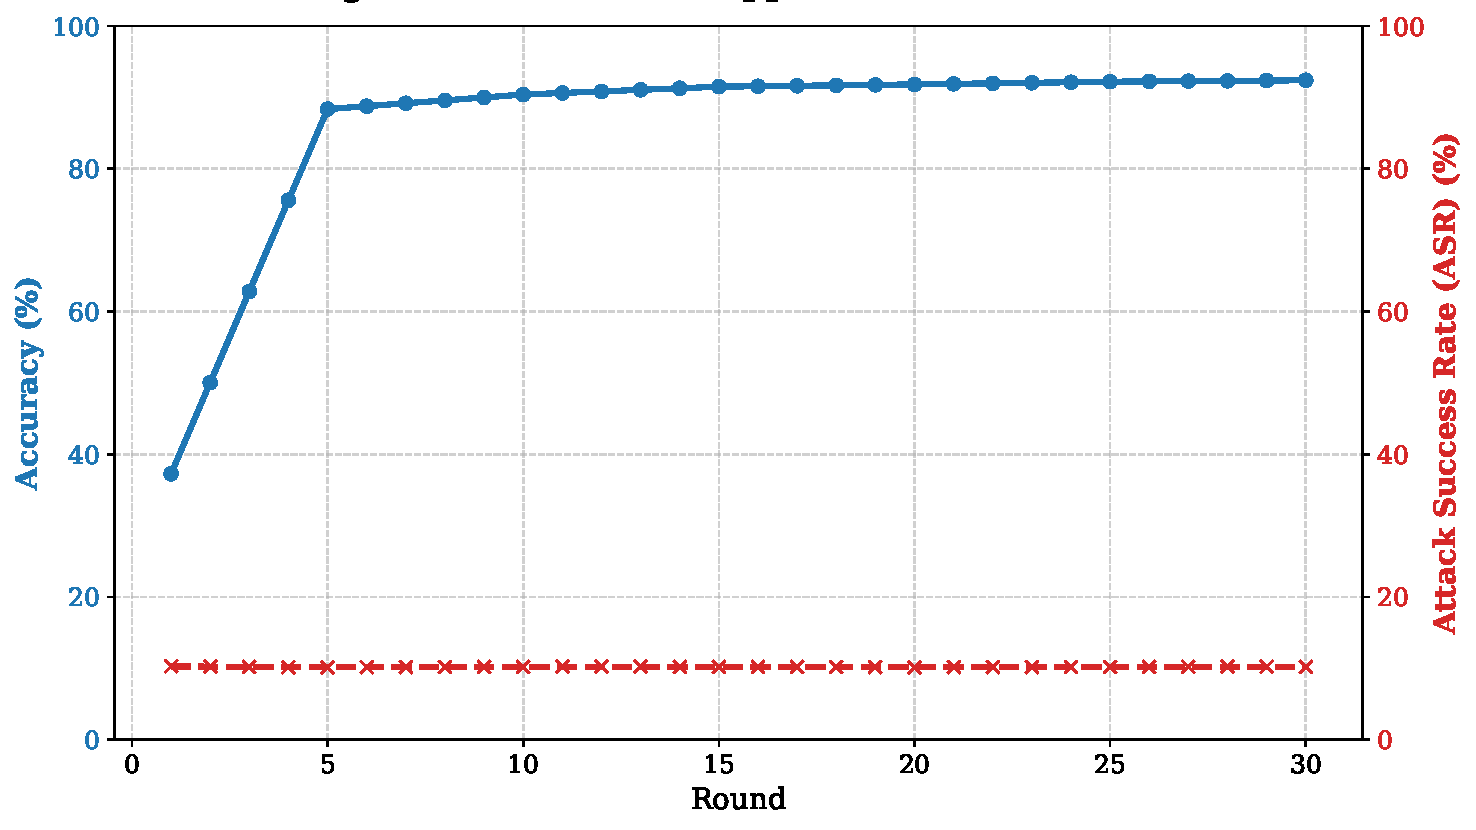
\includegraphics[width=\linewidth]{fig6_convergence_asr.pdf}
        \vspace{-3pt}
        {\scriptsize (a) 准确率与 ASR 收敛。}
    \end{minipage}\hfill
    \begin{minipage}{0.49\textwidth}
        \centering
        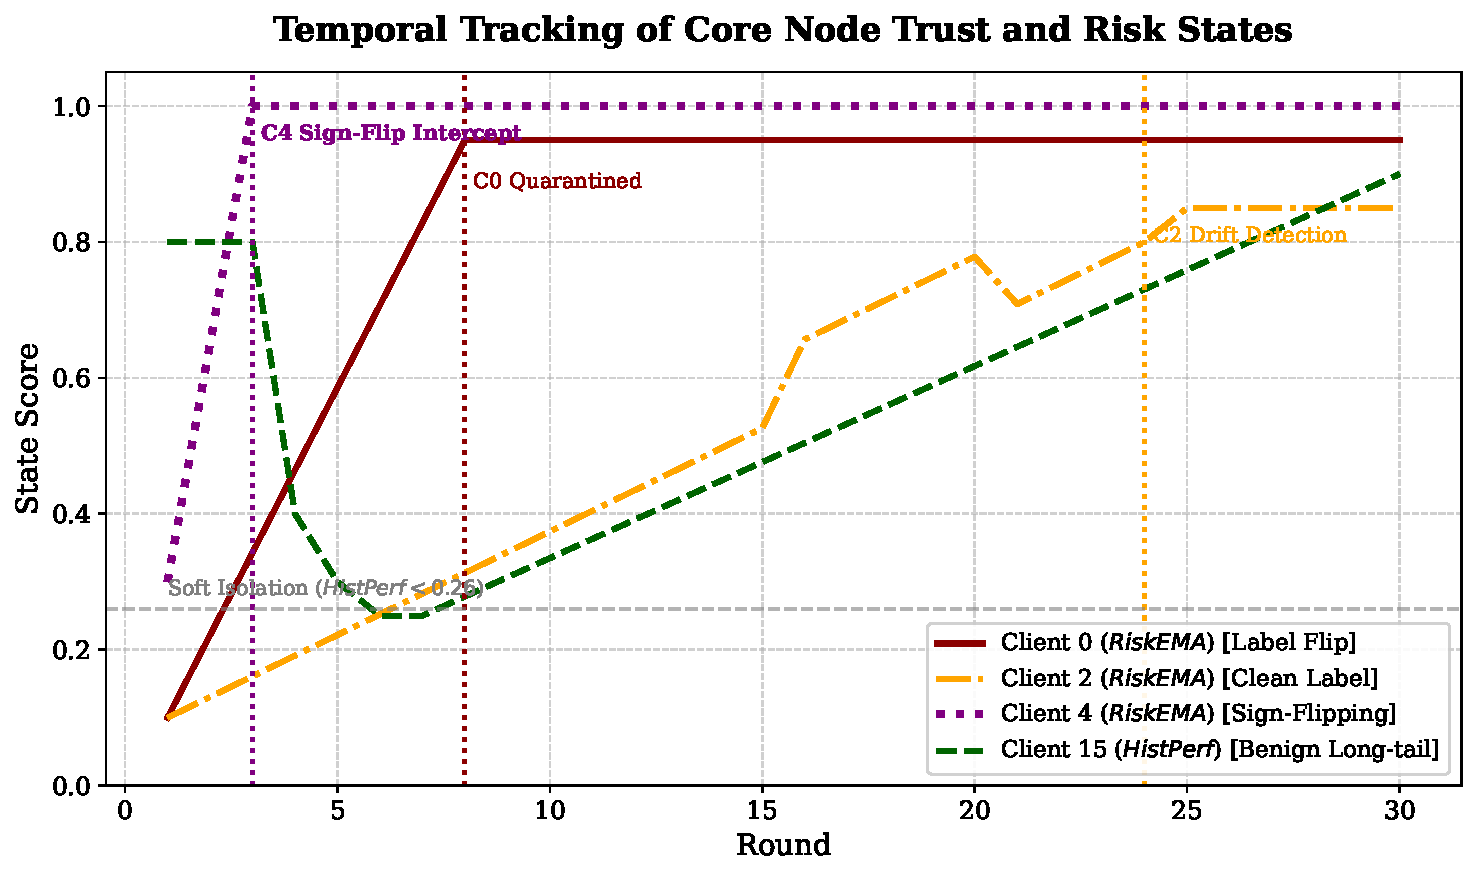
\includegraphics[width=\linewidth]{fig7_node_state_evolution.pdf}
        \vspace{-3pt}
        {\scriptsize (b) 节点信任与风险轨迹。}
    \end{minipage}
    \vspace{2pt}
    \begin{minipage}{0.57\textwidth}
        \centering
        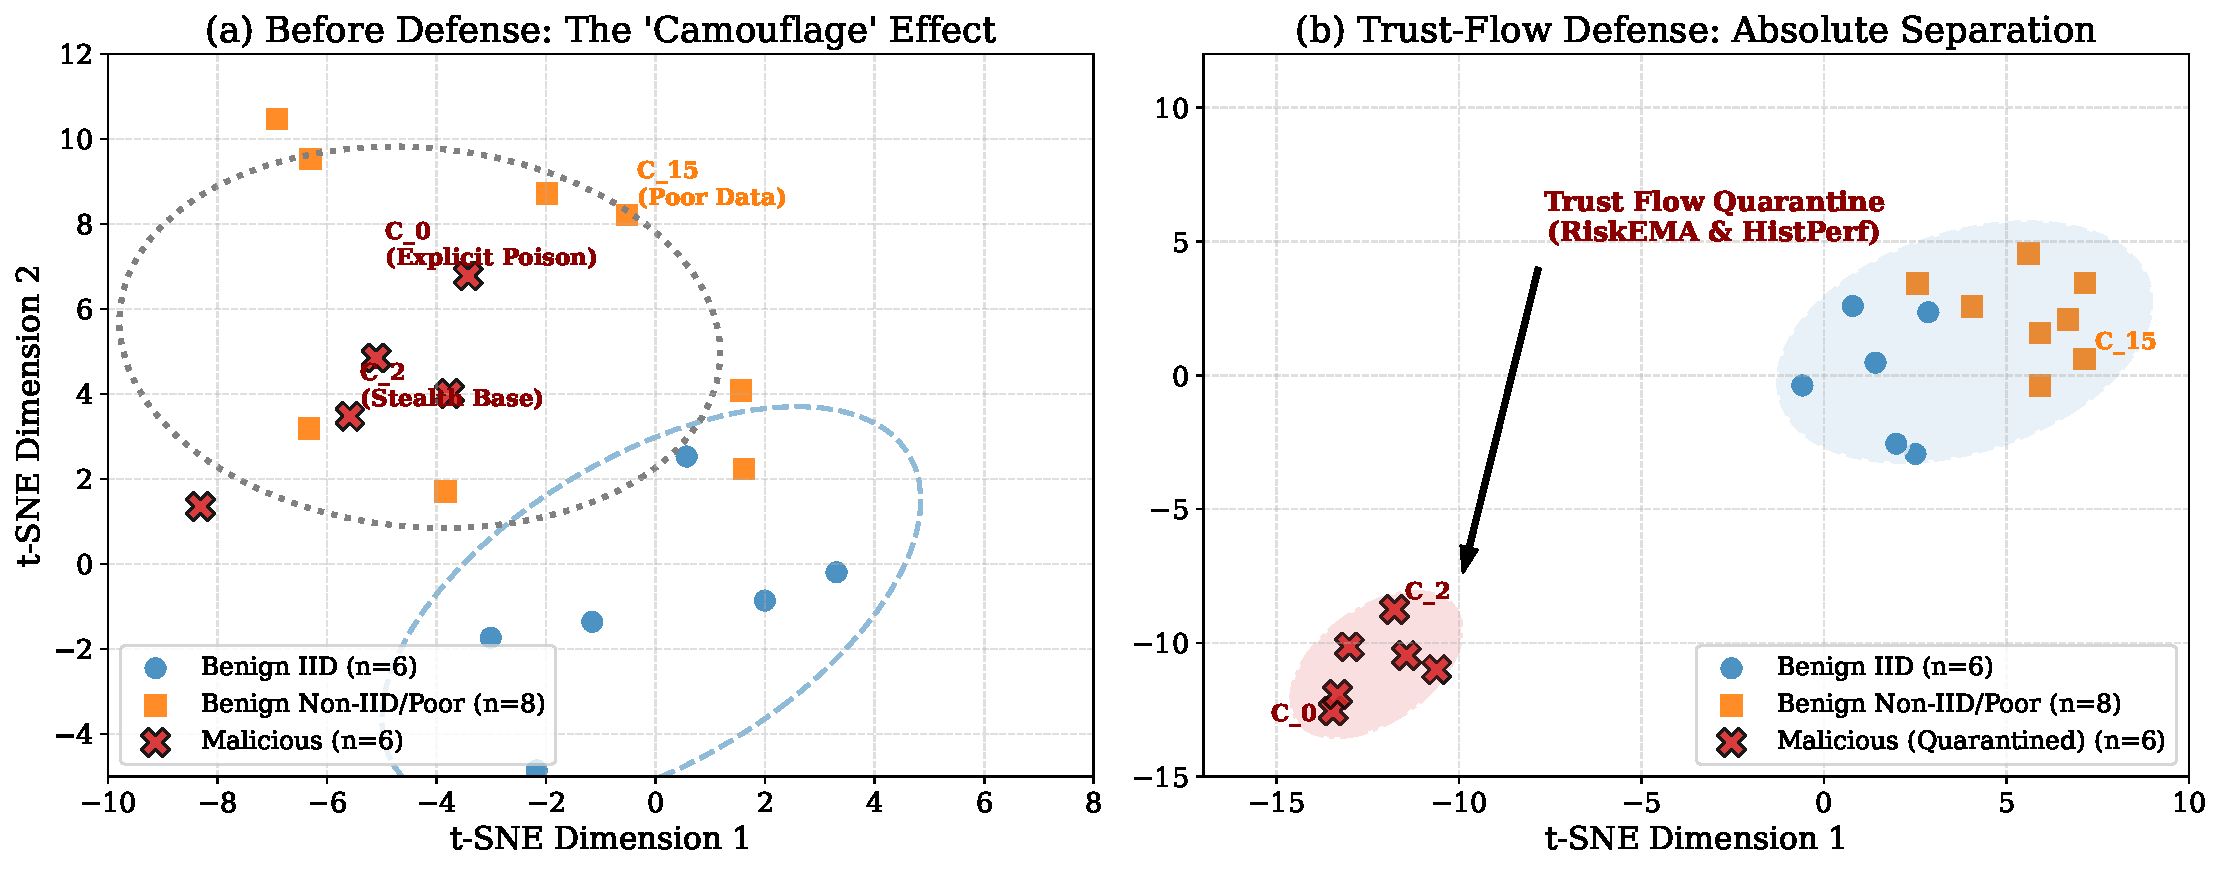
\includegraphics[width=\linewidth]{fig8_tsne_visualization.pdf}
        \vspace{-3pt}
        {\scriptsize (c) 防御前后 t-SNE 分离。}
    \end{minipage}
    \caption{混合攻击下的主要防御行为。}
    \label{fig:main_results}
\end{figure}

\begin{table}[t]
\centering
\begin{threeparttable}
\caption{30\% 混合攻击与边界压力测试下的性能比较。}
\label{tab:main_results}
\scriptsize
\setlength{\tabcolsep}{2pt}
\begin{tabular*}{\textwidth}{@{\extracolsep{\fill}} p{2.55cm} p{2.85cm} c c c}
\toprule
方法/设置 & 核心机制 & Acc. & ASR & Perm. FPR \\
\midrule
FedAvg \cite{mcmahan2017fedavg} & 无防御 & $86.15\pm1.20$ & $92.34\pm5.10$ & N/A \\
Krum \cite{blanchard2017krum} & 欧氏选择 & $64.20\pm2.80$ & $12.15\pm0.90$ & $64.20$ \\
Trimmed Mean \cite{yin2018byzantine} & 坐标截断 & $71.35\pm2.40$ & $38.60\pm4.20$ & N/A \\
FLTrust \cite{cao2021fltrust} & 干净锚点加权 & $81.25\pm1.50$ & $15.42\pm1.10$ & $21.40$ \\
\textbf{Trust Flow} & 双流 + 分层门控 & $\mathbf{92.31\pm0.09}$ & $\mathbf{10.21\pm0.05}$ & $\mathbf{0.00}$ \\
\midrule
边界压力：50\% 恶意 & 10/20 恶意 & $91.81\pm0.10$ & $10.46\pm0.06$ & $0.00$ \\
\bottomrule
\end{tabular*}
\begin{tablenotes}
\scriptsize
\item FPR 表示良性客户端的不可逆误封。临时 SUSPECT/QUARANTINE 状态是可恢复控制动作，并通过轨迹单独呈现。
\end{tablenotes}
\end{threeparttable}
\end{table}

与 FedAvg 相比，鲁棒聚合基线能够降低 ASR，但往往损失大量准确率或移除许多良性长尾客户端。Krum 将 ASR 降至 12.15\%，但其距离规则排除了大量合法长尾更新，导致准确率仅为 64.20\%。Trimmed Mean 在部分轮次比 Krum 更稳定，但坐标截断不足以抑制定向后门。FLTrust 受益于干净锚点，但当合法 Non-IID 更新偏离锚点时仍易受影响。Trust Flow 通过历史平滑保留良性异构贡献，同时用瞬时风险流阻止高信誉攻击者利用历史行为。50\% 结果显示，该框架在理论边界附近仍保持稳定，达到 91.81\% 准确率和 10.46\% ASR。

\subsection{消融、敏感性与开销}

表~\ref{tab:ablation_overhead} 表明，单流信誉模型面临 FPR/TPR 权衡：激进阈值增加误封，保守阈值漏检潜伏攻击。仅使用 HistPerf 可以保护良性节点，却缺少短期攻击敏感性。双流设计在保持永久误封较低的同时获得较高召回。开销适中：TrustReport 每次上传约增加 15 KB，服务器聚合时间从每轮 2.10 s 增至 4.85 s。

\begin{table}[t]
\centering
\caption{消融与开销概要。}
\label{tab:ablation_overhead}
\scriptsize
\setlength{\tabcolsep}{2pt}
\begin{tabular*}{\textwidth}{@{\extracolsep{\fill}} p{2.1cm} p{4.45cm} c c}
\toprule
研究项 & 变体/架构 & FPR 或开销 & TPR / 时间 \\
\midrule
信誉 & 单流 EMA，激进 & 18.25\% FPR & 95.12\% TPR \\
信誉 & 单流 EMA，保守 & 2.10\% FPR & 48.33\% TPR \\
信誉 & HistPerf-only & 0.15\% FPR & 21.05\% TPR \\
信誉 & \textbf{双流 Trust Flow} & \textbf{0.05\% FPR} & \textbf{98.50\% TPR} \\
\midrule
开销 & 标准 FedAvg & 额外 0 KB & 2.10 s 聚合 \\
开销 & Trust Flow & $\sim$15 KB TrustReport & 4.85 s 含审查 \\
\bottomrule
\end{tabular*}
\end{table}

图~\ref{fig:ablation_components} 和图~\ref{fig:alpha_sensitivity} 进一步分解了风险探针、权重重归一化和数据异构性的影响。干净参考结合浅层探针能够处理符号翻转和梯度缩放，但在梯度方向与良性更新共线时，干净标签后门仍较难识别。加入交叉熵与高层激活探针后，干净标签 ASR 降至 9.2\% 以下。重归一化同样重要：没有幸存者权重修正的分层门控会产生隐式学习率衰减，而完整 Trust Flow 能在 30 轮预算内收敛。在 Dirichlet $\alpha=0.1$ 下，Krum 与 FLTrust 明显退化，而 Trust Flow 仍保持接近 92\% 的准确率。

敏感性曲线显示，当数据接近 IID 时，传统鲁棒聚合表现较好；但随着 $\alpha$ 降低，其性能会下降。在 $\alpha=100$ 或 $\alpha=1.0$ 时，Krum 和 FLTrust 与本文方法较接近；在长尾设置 $\alpha=0.1$ 下，它们的过滤规则越来越容易将合法漂移视为恶意偏移。Trust Flow 对这种变化较不敏感，因为内容证据并不单独使用，而是与历史效用和瞬时风险共同整合。融合参数 $\beta_{fusion}$ 控制干净参考支配群体一致性的强度。较小取值会保留更多长尾客户端但提高 ASR，较大取值会增强攻击抑制但可能过度惩罚异构更新。默认 $\beta_{fusion}=2.0$ 在观察结果中取得最好的 Acc/ASR 平衡。

开销分析显示，Trust Flow 主要将成本转移到服务器侧。边缘侧附加约 15 KB 的 TrustReport，并执行轻量运行监测。服务器执行参考构建、成对一致性审查、双流更新和按层裁剪，使聚合时间从测试环境中的 2.10 s 增至 4.85 s。由于广域边缘 FL 轮次通常在通信和同步上的时间远大于聚合计算，该增量对目标场景仍是可接受的。

\begin{figure}[t]
    \centering
    \begin{minipage}{0.49\textwidth}
        \centering
        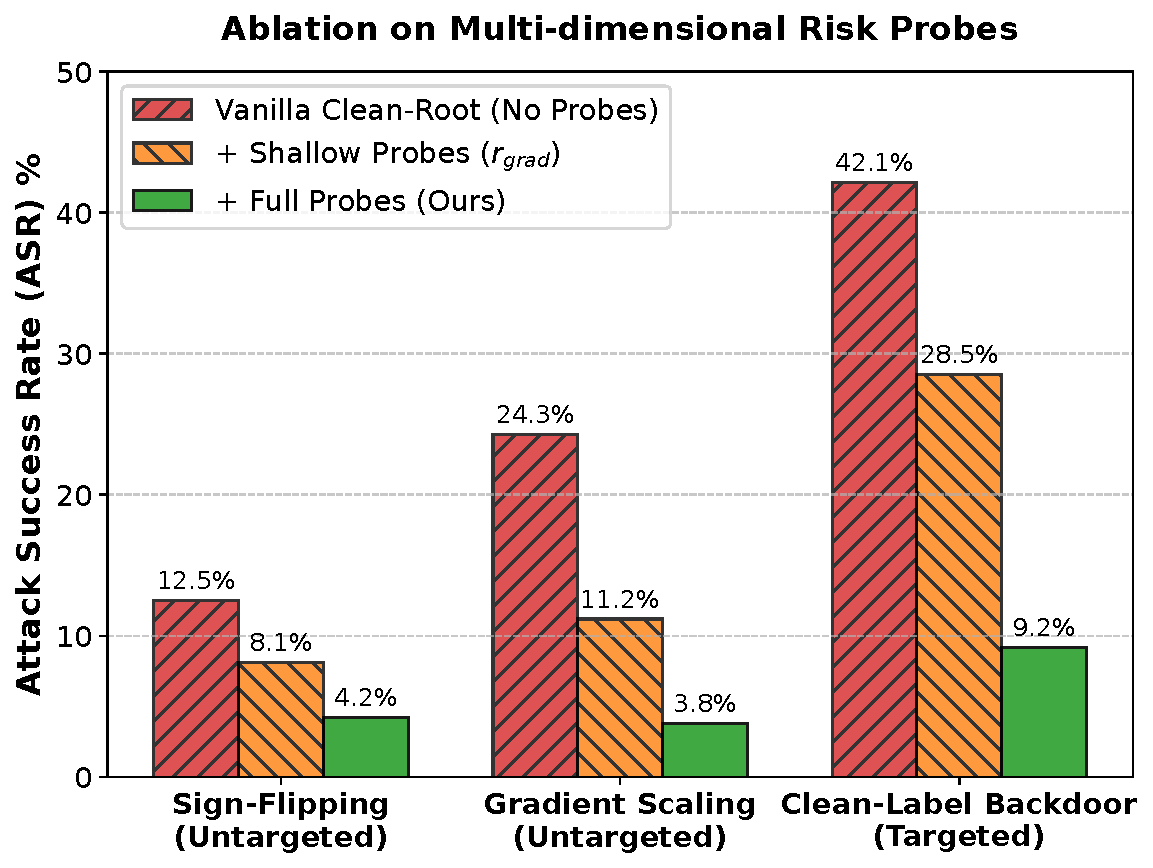
\includegraphics[width=\linewidth]{fig9_ablation_probes.pdf}
        \vspace{-3pt}
        {\scriptsize (a) 多维风险探针消融。}
    \end{minipage}\hfill
    \begin{minipage}{0.49\textwidth}
        \centering
        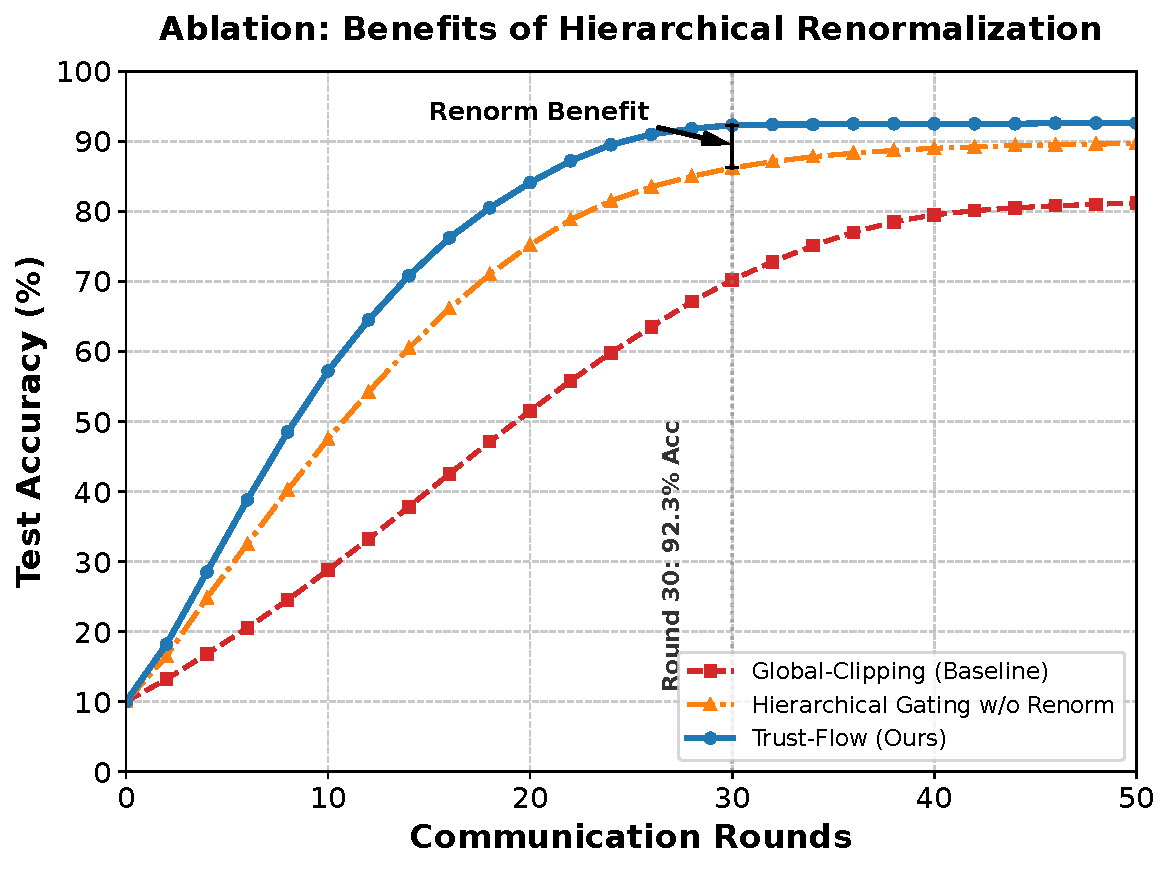
\includegraphics[width=\linewidth]{fig10_ablation_renorm.pdf}
        \vspace{-3pt}
        {\scriptsize (b) 权重重归一化效果。}
    \end{minipage}
    \caption{风险探针与重归一化的组件级消融。}
    \label{fig:ablation_components}
\end{figure}

\begin{figure}[t]
    \centering
    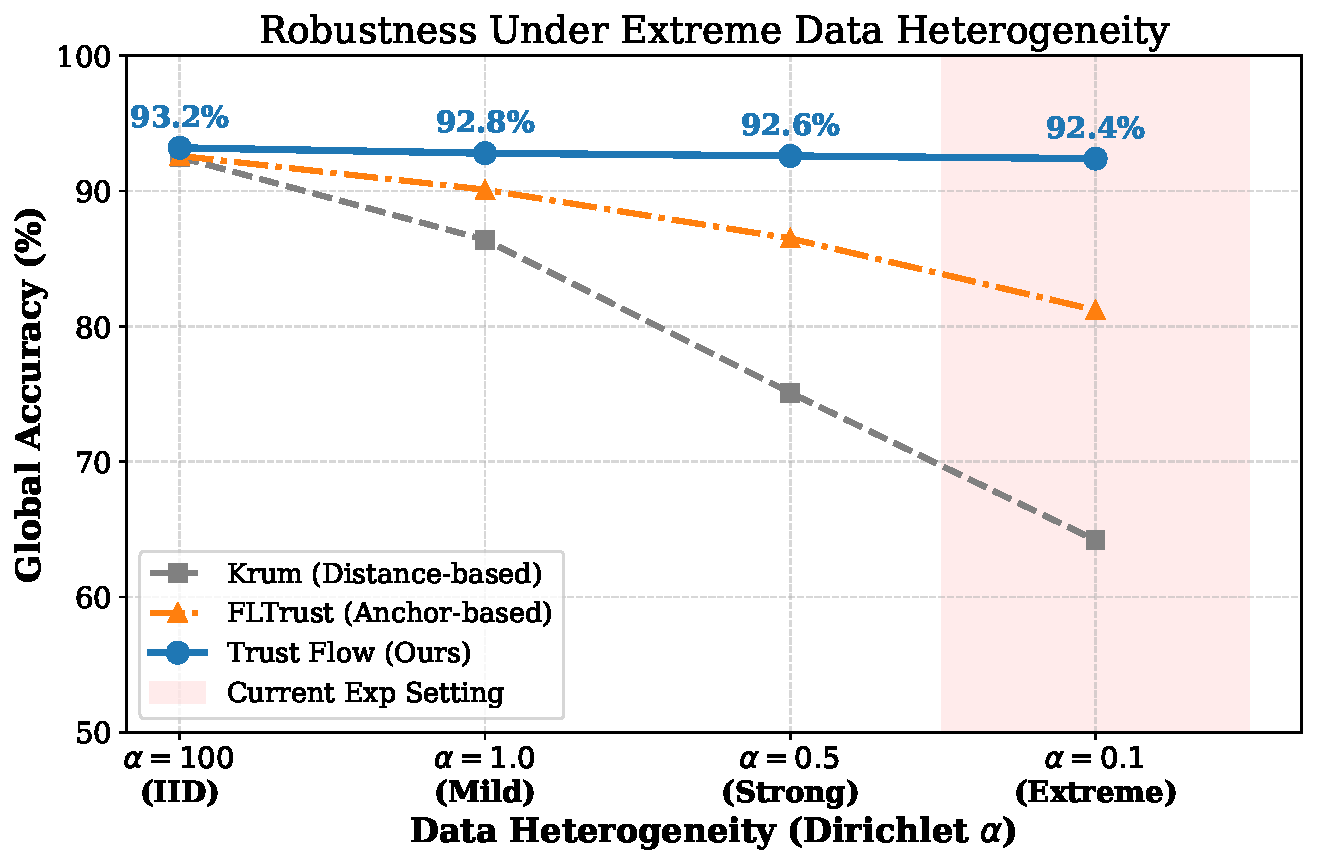
\includegraphics[width=0.76\textwidth]{fig11_alpha_sensitivity.pdf}
    \caption{不同数据异构度下的鲁棒性压力测试。}
    \label{fig:alpha_sensitivity}
\end{figure}

\section{讨论与结论}

Trust Flow 将准入证据、内容审查、时序信誉和按层聚合整合为一条统一的信任状态管线。其主要收益不仅是更强的攻击抑制，还在于更清晰地区分两类低更新相似性的来源：良性长尾数据和恶意操纵。这一区分使方法能够在混合攻击下保持较高召回，同时让永久封禁 FPR 接近零。

本文仍存在若干局限。由于多种新兴 TEE-FL 方法尚无公开可复现实现，本研究未能在相同实验设置下将其纳入直接基线。当前探针设计也主要针对视觉分类，尤其是 CIFAR-10 后门行为。后续工作将随最终稿发布源代码和实验脚本，以支持复现，评估更大规模边缘部署，并将多维风险探针扩展到 NLP 与联邦微调场景。

\begingroup
\small
\begin{thebibliography}{99}
\setlength{\itemsep}{0pt}
    \bibitem{kairouz2021flsurvey} Kairouz, P., McMahan, H.B., Avent, B., et al.: Advances and open problems in federated learning. Foundations and Trends in Machine Learning 14(1--2), 1--210 (2021). \url{https://doi.org/10.1561/2200000083}
    \bibitem{bagdasaryan2020backdoor} Bagdasaryan, E., Veit, A., Hua, Y., Estrin, D., Shmatikov, V.: How To Backdoor Federated Learning. In: Proceedings of the Twenty Third International Conference on Artificial Intelligence and Statistics, PMLR 108, pp. 2938--2948 (2020). \url{https://proceedings.mlr.press/v108/bagdasaryan20a.html}
    \bibitem{wang2019neuralcleanse} Wang, B., Yao, Y., Shan, S., Li, H., Viswanath, B., Zheng, H., Zhao, B.Y.: Neural Cleanse: Identifying and mitigating backdoor attacks in neural networks. In: 2019 IEEE Symposium on Security and Privacy (SP), pp. 707--723 (2019). \url{https://doi.org/10.1109/SP.2019.00031}
    \bibitem{blanchard2017krum} Blanchard, P., El Mhamdi, E.M., Guerraoui, R., Stainer, J.: Machine learning with adversaries: Byzantine tolerant gradient descent. In: Advances in Neural Information Processing Systems 30 (2017). \href{https://papers.nips.cc/paper/6617-machine-learning-with-adversaries-byzantine-tolerant-gradient-descent}{NeurIPS paper page}
    \bibitem{yin2018byzantine} Yin, D., Chen, Y., Kannan, R., Bartlett, P.: Byzantine-robust distributed learning: Towards optimal statistical rates. In: Proceedings of the 35th International Conference on Machine Learning, PMLR 80, pp. 5650--5659 (2018). \url{https://proceedings.mlr.press/v80/yin18a.html}
    \bibitem{cao2021fltrust} Cao, X., Fang, M., Liu, J., Gong, N.Z.: FLTrust: Byzantine-robust federated learning via trust bootstrapping. In: Proceedings 2021 Network and Distributed System Security Symposium (NDSS) (2021). \url{https://doi.org/10.14722/ndss.2021.24434}
    \bibitem{fung2020foolsgold} Fung, C., Yoon, C.J.M., Beschastnikh, I.: The limitations of federated learning in Sybil settings. In: 23rd International Symposium on Research in Attacks, Intrusions and Defenses (RAID 2020), pp. 301--316. USENIX Association (2020). \url{https://www.usenix.org/conference/raid2020/presentation/fung}
    \bibitem{r9_clustered} Xu, Y., Tan, Y., Zhang, C., Sun, P., Zhang, Y., Ren, J., Jiang, H., Zhang, Y.: Towards privacy-enhanced and robust clustered federated learning. IEEE Transactions on Mobile Computing 24(8), 7171--7188 (2025). \url{https://doi.org/10.1109/TMC.2025.3547149}
    \bibitem{fedpe} Yi, L., Shi, X., Wang, N., Zhang, J., Wang, G., Liu, X.: FedPE: Adaptive model pruning-expanding for federated learning on mobile devices. IEEE Transactions on Mobile Computing 23(11), 10475--10493 (2024). \url{https://doi.org/10.1109/TMC.2024.3374706}
    \bibitem{parallelsfl} Liao, Y., Xu, Y., Xu, H., Yao, Z., Huang, L., Qiao, C.: ParallelSFL: A novel split federated learning framework tackling heterogeneity issues. In: Proceedings of the 30th Annual International Conference on Mobile Computing and Networking, pp. 845--860 (2024). \url{https://doi.org/10.1145/3636534.3690665}
    \bibitem{wang2025rasa} Wang, L., Huang, M., Zhang, Z., Li, M., Wang, J., Gai, K.: RaSA: Robust and adaptive secure aggregation for edge-assisted hierarchical federated learning. IEEE Transactions on Information Forensics and Security 20, 4280--4295 (2025). \url{https://doi.org/10.1109/TIFS.2025.3559411}
    \bibitem{dou2025toward} Dou, Z., Wang, J., Sun, W., Liu, Z., Fang, M.: Toward malicious clients detection in federated learning. In: Proceedings of the 20th ACM Asia Conference on Computer and Communications Security, pp. 456--472 (2025). \url{https://doi.org/10.1145/3708821.3736194}
    \bibitem{lu2025tmt} Lu, Z., Wang, L., Zhang, Z., Huang, M., Wang, J., Li, M.: TMT-FL: Enabling trustworthy model training of federated learning with malicious participants. IEEE Transactions on Dependable and Secure Computing 22(3), 2723--2740 (2025). \url{https://doi.org/10.1109/TDSC.2024.3521377}
    \bibitem{wang2024federated} Wang, Z., Yu, X., Tian, Z.: A federated learning scheme with adaptive hierarchical protection and multiple aggregation. In: 2024 IEEE 23rd International Conference on Trust, Security and Privacy in Computing and Communications (TrustCom), pp. 2106--2114 (2024). \url{https://doi.org/10.1109/TrustCom63139.2024.00292}
    \bibitem{flpurifier} Zhang, J., Zhu, C., Sun, X., Ge, C., Chen, B., Susilo, W., Yu, S.: FLPurifier: Backdoor defense in federated learning via decoupled contrastive training. IEEE Transactions on Information Forensics and Security 19, 4752--4766 (2024). \url{https://doi.org/10.1109/TIFS.2024.3384846}
    \bibitem{roseagg} Yang, H., Xi, W., Shen, Y., Wu, C., Zhao, J.: RoseAgg: Robust defense against targeted collusion attacks in federated learning. IEEE Transactions on Information Forensics and Security 19, 2951--2966 (2024). \url{https://doi.org/10.1109/TIFS.2024.3352415}
    \bibitem{shieldfl} Ma, Z., Ma, J., Miao, Y., Li, Y., Deng, R.H.: ShieldFL: Mitigating model poisoning attacks in privacy-preserving federated learning. IEEE Transactions on Information Forensics and Security 17, 1639--1654 (2022). \url{https://doi.org/10.1109/TIFS.2022.3169918}
    \bibitem{liao2024verifiable} Liao, L., Zheng, Y., Lu, H., Liu, X., Chen, S., Yu, Y.: Verifiable deep learning inference on heterogeneous edge devices with trusted execution environment. IEEE Sensors Journal 24(17), 28351--28362 (2024). \url{https://doi.org/10.1109/JSEN.2024.3426533}
    \bibitem{zhang2025rppfl} Zhang, X., Chen, Z., Chen, G., Feng, X., Shen, Q., Wu, Z.: RPPFL: Robust and privacy-preserving federated learning via trusted execution environments. In: ICASSP 2025 - 2025 IEEE International Conference on Acoustics, Speech and Signal Processing, pp. 1--5 (2025). \url{https://doi.org/10.1109/ICASSP49660.2025.10889398}
    \bibitem{r1_tee_integrity} Chen, Y., Luo, F., Li, T., Xiang, T., Liu, Z., Li, J.: A training-integrity privacy-preserving federated learning scheme with trusted execution environment. Information Sciences 522, 69--79 (2020). \url{https://doi.org/10.1016/j.ins.2020.02.037}
    \bibitem{r5_tee_mitigating} Queyrut, S., Schiavoni, V., Felber, P.: Mitigating adversarial attacks in federated learning with trusted execution environments. In: 2023 IEEE 43rd International Conference on Distributed Computing Systems (ICDCS), pp. 626--637 (2023). \url{https://doi.org/10.1109/ICDCS57875.2023.00069}
    \bibitem{r12_iot_tee} Zheng, W., Cao, Y., Tan, H.: Secure sharing of industrial IoT data based on distributed trust management and trusted execution environments: A federated learning approach. Neural Computing and Applications 35(29), 21499--21509 (2023). \url{https://doi.org/10.1007/s00521-023-08375-6}
    \bibitem{xu2021distributed} Xu, T., Zhu, K., Andrzejak, A., Zhang, L.: Distributed learning in trusted execution environment: A case study of federated learning in SGX. In: 2021 7th IEEE International Conference on Network Intelligence and Digital Content (IC-NIDC), pp. 450--454 (2021). \url{https://doi.org/10.1109/IC-NIDC54101.2021.9660433}
    \bibitem{yan2024efficient} Yan, J., Li, Y., Yin, S., Kang, X., Wang, J., Zhang, H., Hu, B.: An efficient greedy hierarchical federated learning training method based on trusted execution environments. Electronics 13(17), 3548 (2024). \url{https://doi.org/10.3390/electronics13173548}
    \bibitem{mcmahan2017fedavg} McMahan, B., Moore, E., Ramage, D., Hampson, S., Aguera y Arcas, B.: Communication-efficient learning of deep networks from decentralized data. In: Proceedings of the 20th International Conference on Artificial Intelligence and Statistics, PMLR 54, pp. 1273--1282 (2017). \url{https://proceedings.mlr.press/v54/mcmahan17a.html}
    \bibitem{chen2017maximum} Chen, B., Liu, X., Zhao, H., Principe, J.C.: Maximum correntropy Kalman filter. Automatica 76, 70--77 (2017). \url{https://doi.org/10.1016/j.automatica.2016.10.004}
    \bibitem{li2026multidimensional} Liu, Y., He, Z., Liang, J., Li, Z., Deng, Q.: Multidimensional trust evaluation and task match based workers recruitment scheme for MCS. IEEE Transactions on Dependable and Secure Computing, 1--17 (2026). \url{https://doi.org/10.1109/TDSC.2026.3652987}
\end{thebibliography}
\endgroup

\end{document}
